\documentclass[hidelinks]{article}
\usepackage[T2A]{fontenc}
\usepackage[utf8]{inputenc}
\usepackage[russian]{babel}
\usepackage{graphicx}
\usepackage[export]{adjustbox}
\usepackage{geometry}
\usepackage{float}
\usepackage{indentfirst}
\usepackage{listings}
\usepackage{hyperref}

\begin{document}

\include{title_page}
\tableofcontents
\pagebreak

\section{Введение}
В настоящее время всё большую популярность приобретают различные интернет-сервисы, в том числе и браузерные игры. Одной из таких является игра 2048. Игровое поле этой игры имеет форму квадрата 4x4. Целью игры является получение плитки номинала «2048». 

В настоящей работе рассматривается создание аналога этой игры с возможностью просмотра таблицы рекордов.

\section{Постановка задачи}
Была поставлена задача разработать web-версию игры 2048. 

Данное приложение должно предоставлять следующую функциональность: 
\begin{enumerate}
    \item Обеспечить возможность регистрации пользователя 
    \item Обеспечить возможность входа на сайт зарегистрированного пользователя 
    \item Играть в игру 2048 
    \item Просматривать таблицу рекордов игроков 
\end{enumerate}

\section{Метод решения задачи}
Принято решение разделить приложение на 2 части: серверную и клиентскую.
Взаимодействие между клиентом и сервером будет осуществляться посредством протокола HTTP и подхода REST.

Сервер будет предоставлять открытый API, с которым клиент будет взаимодействовать, передавая или получая необходимую информацию.

Для хранения данных будет использоваться база данных, с которой будет взаимодействовать сервер.

Схема базы данных приложения представлена на рисунке \ref{fig:db}.

\begin{figure}[H]
    \centering
    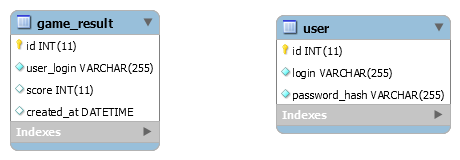
\includegraphics[scale=0.5]{img/db.png}
    \caption{Схема базы данных}
    \label{fig:db}
\end{figure}

На данной схеме присутствуют следующие таблицы:
\begin{enumerate}
    \item user - данная таблица необходима для хранения пользователей.

    Атрибуты таблицы:
    \begin{enumerate}
        \item id - первичный ключ
        \item login - имя пользователя
        \item password\_hash - пароль пользователя
    \end{enumerate}
    \item game\_result - данная таблица хранит рекорды пользователей.
    
    Атрибуты таблицы:
    \begin{enumerate}
        \item id - первичный ключ
        \item user\_login - имя пользователя
        \item score - количество набранных очков
        \item created\_at - дата игры
    \end{enumerate}
\end{enumerate}

\section{Средства реализации}
Выбор программных средств для реализации приложения частично определен тем, программным обеспечением, которое доступно на сервере, на котором это приложение будет расположено.

\textbf{Серверная часть}
\begin{enumerate}
    \item Язык программирования: Python 3
    \item Bottle - микрофреймворк для построения веб приложений
    \item Различные плагины для Bottle, добавляющие нужную функциональность
\end{enumerate}

\textbf{Клиентская часть}
\begin{enumerate}
    \item Язык программирования: TypeScript, HTML, CSS
    \item Angular 7 - популярный фреймворк от Google для построения динамических одностраничных приложений
    \item Bulma - легковесный CSS фреймворк
\end{enumerate}

\textbf{СУБД:} MySQL

\textbf{Web-сервер:} Apache

\section{Схема работы приложения}
Весь процесс от момента нажатия пользователем на кнопку до получения какого-либо отклика можно описать схемой \ref{fig:sequence}.


\begin{figure}[H]
    \centering
    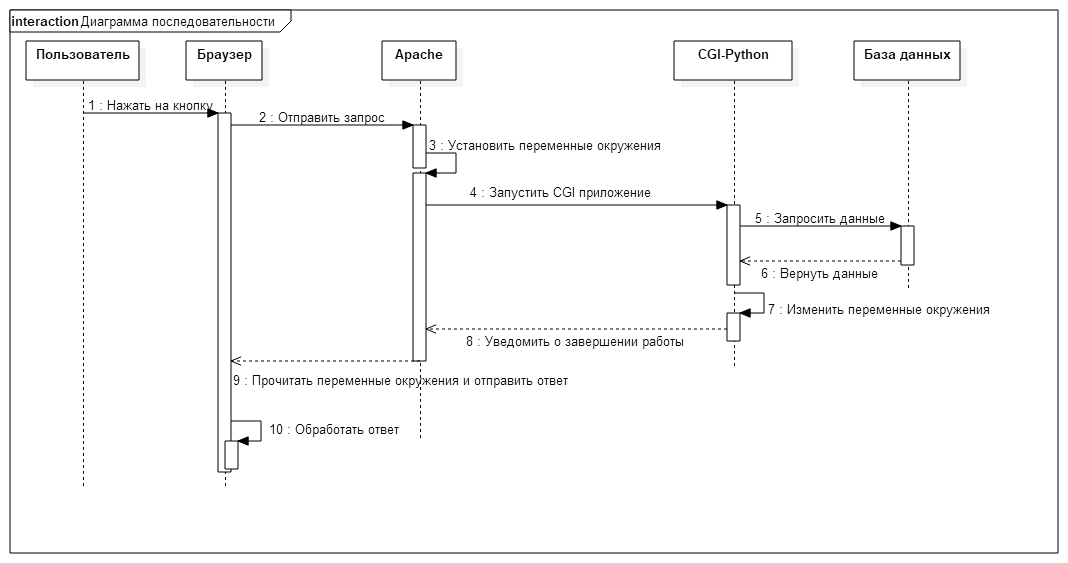
\includegraphics[width=\textwidth]{img/sequence.png}
    \caption{Диаграмма последовательности}
    \label{fig:sequence}
\end{figure}

Если пользователь совершает какое-то действие, которое требует участие сервера (например, переход на страницу с рекордами), то браузер посылает соответствующий запрос.

Веб-сервер Apache принимает этот запрос и устанавливает некоторые переменные окружения, которые могут далее быть прочитаны приложением. Когда переменные установлены, запускается CGI скрипт, который в данном случае вызывает интерепретатор Python и запускает само приложение.

Python-приложение читает переменные окружения и получает оттуда информацию о запросе и выполняет необходимые действия, соответствующие запросу. Если это был запрос таблицы рекордов, то сервер обращается к MySQL базе данных и получает от нее нужные данные, сериализует их в JSON формат, записывает ответ в переменные окружения и завершает свою работу.

Когда приложение завершило работу, Apache читает измененные переменные окружения и отправляет браузеру ответ.

Браузер принимает ответ и обрабатывает его. Если это был запрос на таблицу рекордов, то открывается соответствующая страница, где отображается таблица с записями.


\section{Пользовательский интерфейс}

Форма входа представлена на рисунке \ref{fig:signin}. 

Полями данной формы являются логин и пароль пользователя. После того, как оба поля будут заполнены, кнопка Войти станет активной.

\begin{figure}[H]
    \centering
    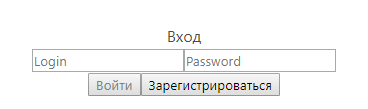
\includegraphics[]{img/signin.png}
    \caption{Страница входа}
    \label{fig:signin}
\end{figure}

Если у пользователя нет аккаунта, он может нажать на кнопку Зарегистрироваться, после чего откроется форма регистрации, представленная на рисунке \ref{fig:signup}.

После того, как оба поля (логин и пароль) будут заполнены, кнопка Зарегистрироваться станет активной.

\begin{figure}[H]
    \centering
    
\includegraphics[]{img/signup.png}
    \caption{Страница регистрации}
    \label{fig:signup}
\end{figure}

Главная страница пользовательского интерфейса представлена на рисунке \ref{fig:main}. 

На этой странице расположено поле с игрой и следующие пункты меню:
\begin{enumerate}
    \item Новая игра - сохраняет текущие очки пользователя в таблицу с рекордами и начинает новую игру
    \item Игра - переходит на страницу с игрой
    \item Рекорды - переходит на страницу с рекордами
    \item Выйти - выйти из аккаунта
\end{enumerate}

\begin{figure}[H]
    \centering
    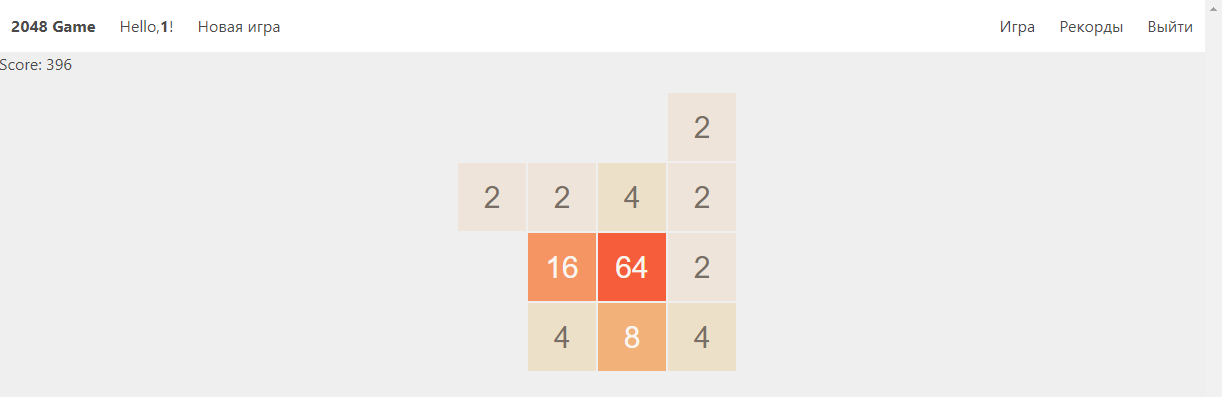
\includegraphics[scale=0.5]{img/game.png}
    \caption{Главная страница}
    \label{fig:main}
\end{figure}

Страница с таблицами рекордов представлена на рисунке \ref{fig:leaderboards}.

В данной таблице отображена информация о законченной игре: имя игрока, очки и дата игры.

\begin{figure}[H]
    \centering
    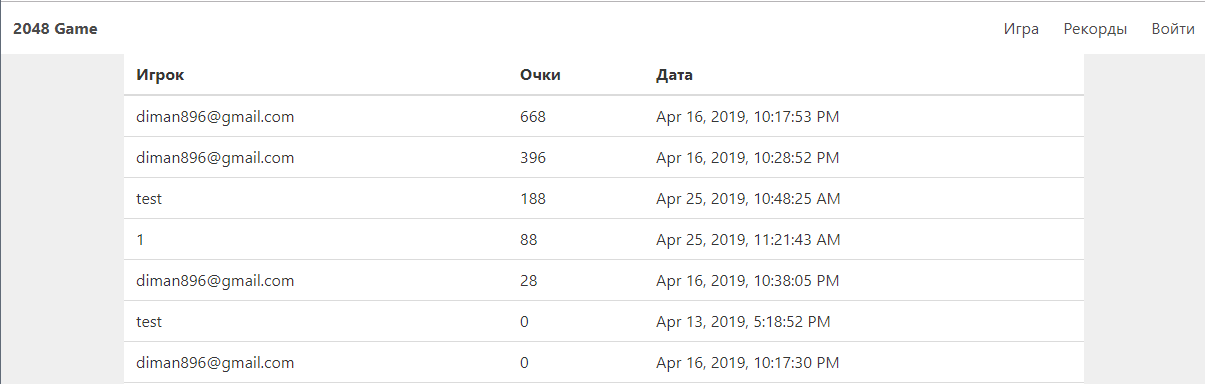
\includegraphics[scale=0.5]{img/leaderboards.png}
    \caption{Таблица рекордов}
    \label{fig:leaderboards}
\end{figure}


\section{Оценка степени завершенности и перспективы доработки проекта}
На данном этапе разработки приложение является законченным, оно полностью удовлетворяет всем поставленным требованиям. Доработка приложения не требуется, но возможна.

Например, возможными направлениями для доработки могут быть:
\begin{enumerate}
    \item Создание графика с личными рекордами
    \item Создание сравнительных графиков рекордов нескольких пользователей
\end{enumerate}

\section{Хронология проделанной работы}
\begin{enumerate}
    \item Разработана логика самой игры на клиентской стороне
    \item Разработана серверная часть, которая включает в себя логику сервера и модель базы данных (которая создана при помощи Code-First подхода)
    \item На клиентской стороне реализована логика взаимодействия с серверной частью
    \item Проведено ручное тестирование всей функциональности
    \item Клиентское и серверное приложения развернуты на веб-сервере ФКН
    \item Проведено ручное тестирование функциональности приложения на сервере ФКН, исправлены ошибки, которые появились на новом окружении
\end{enumerate}

\section{Заключение}
Результатом работы является приложение для игры 2048, предоставляющее следующую функциональность:
\begin{enumerate}
    \item Обеспечение возможности регистрации пользователя 
    \item Обеспечение возможности входа на сайт зарегистрированного пользователя 
    \item Предоставление возможности играть в игру 2048 
    \item Просмотр таблицы рекордов игроков 
\end{enumerate}

\section{Приложение}
Полный исходный код приложения расположен по адреcy:

\url{http://www2/~vychikov_d_d/2048.zip}  

\end{document}
